\chapter{Analyse}
\label{sec:analyse}
Zusätzlich zu den maschinellen Lernkomponenten stellt Unity auch Demonstrationsumgebungen bereit, in denen verschiedene Lösungen für gängige Verstärkungslernprobleme implementiert sind. In der Walker-Demo wird ein physisch simulierter Charakter darauf trainiert, zu einem Zielwürfel zu laufen. Sie implementiert bereits einige grundlegende Steuerungsmechanismen, die erforderlich sind, um einen Charakter in einer dynamischen Umgebung zu bewegen und zu kontrollieren. Aus diesem Grund wird in dieser Arbeit die Walker-Demo als Basis für die Entwicklung genutzt. 

In diesem Kapitel wird daher die Walker-Demo analysiert, um in den folgenden Kapiteln darauf aufzubauen. Es wird untersucht wie die Szene und der Charakter aufgebaut sind, welche Beobachtungen als Eingabe verwendet werden und wie Ausgabe des neuronalen Netz in der Umgebung ausgeführt werden. Anschließend wird der Ablauf und die verwendete Belohnungsfunktion analysiert.

\section{Szenenaufbau}
Die Szene besteht aus einem quadratischen Spielfeld mit einem Boden und Wänden, die der Charakter nicht verlassen kann (siehe Abbildung \ref{fig:walker_aufbau}). Diese Begrenzungen dienen dazu, die Bewegung des Charakters zu kontrollieren und sicherzustellen, dass die Lernumgebung konsistent bleibt. Die Umgebung umfasst weiterhin den Läufer und das Ziel, zu dem der Läufer lernt zu laufen.

\begin{figure}[H]
  \centering  
  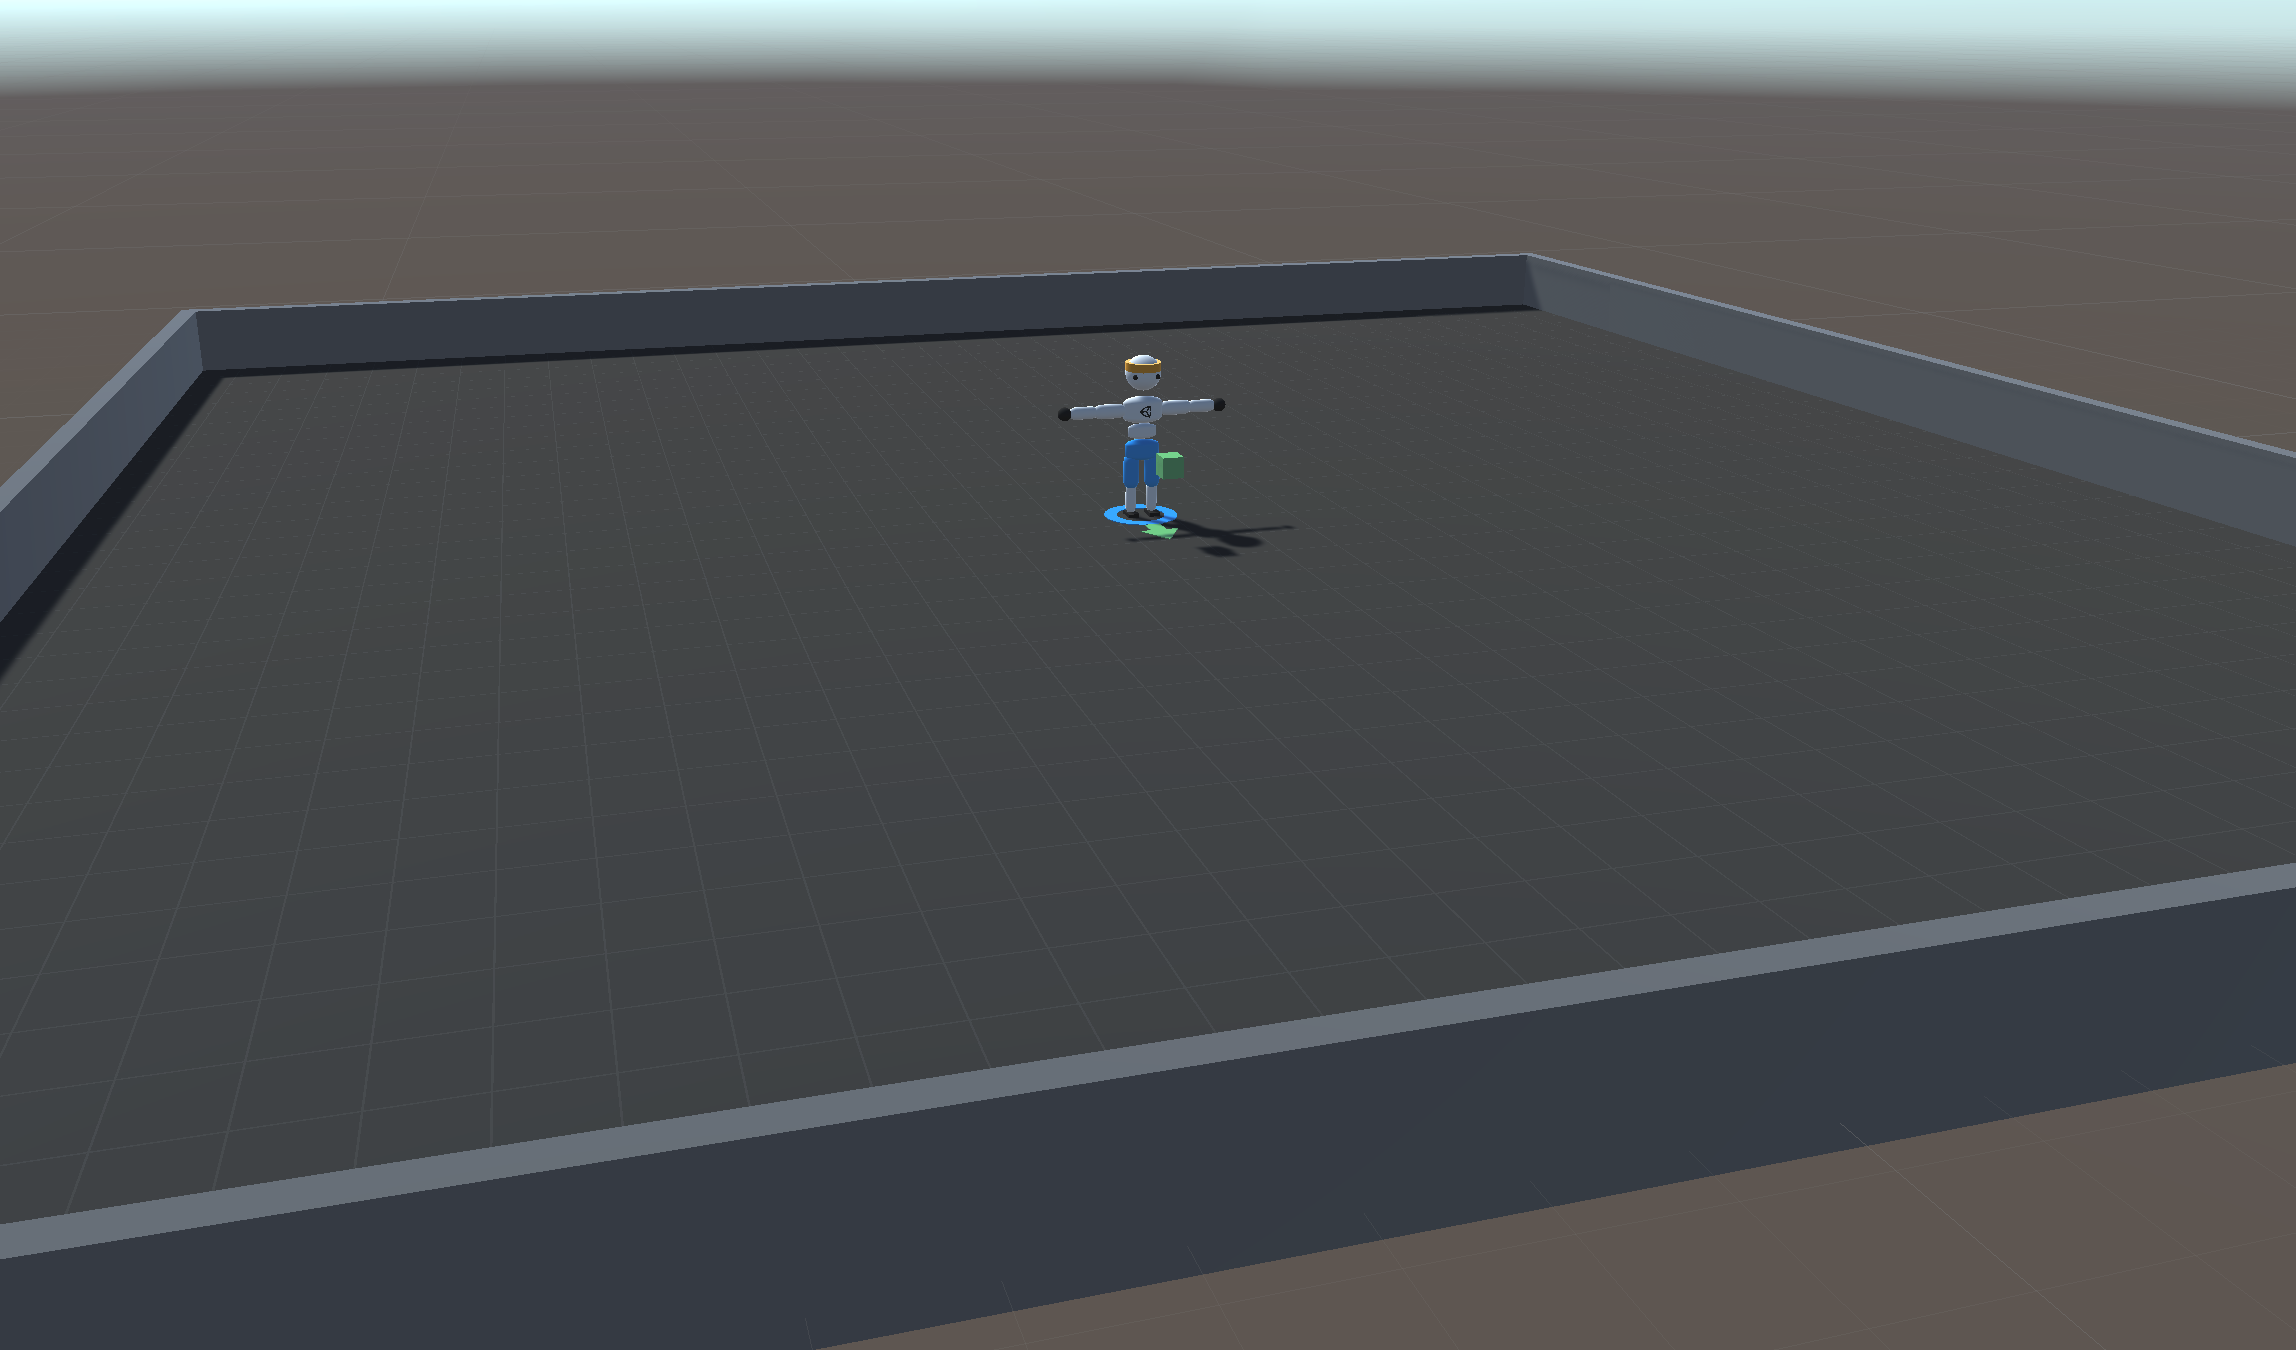
\includegraphics[scale=0.35]{img/walker_aufbau.png}
  \caption{Walker-Demo Szenenaufbau}
  \label{fig:walker_aufbau}
\end{figure}

\section{Läufer}
Der Körper des Läufers ist sorgfältig mit verschiedenen geometrischen Formen aufgebaut: 11 Kapseln, drei Kugeln und zwei Quadern. Jede dieser Formen verfügt über eine Festkörper- und eine Kollisions-Physikkomponente, die eine realistische Interaktion innerhalb der Szene ermöglichen. Die Gelenke zwischen den Körperteilen werden als Kugelgelenke simuliert, um eine flexible und natürliche Bewegung zu gewährleisten.

Die genaue Physikkonfiguration der Körperteile wird in der Tabelle \ref{table:walker_körperteile} veranschaulicht. Diese Konfiguration spielt eine zentrale Rolle, da sie die Art und Weise bestimmt, wie der Läufer lernt, auf das Ziel zuzulaufen, und dabei die physischen Einschränkungen und Möglichkeiten berücksichtigt.

\begin{table}[H]
  \centering
  {\rowcolors{1}{gray!10}{white}
  \begin{tabular}{ |p{3cm}|p{3cm}|p{2cm}|p{4cm}|p{2cm}| }
  \hline
  \textbf{Körpertei}l& \textbf{Verbundenes Körperteil} & \textbf{Gewicht} & \textbf{Winkellimits} & \textbf{Form} \\
  \hline
  Hüfte & - & 15kg & - & Kapsel \\
  \hline
  Wirbelsäule & Hüfte & 10kg & x(-20,20) y(-20,20) z(-15,15) & Kapsel \\
  \hline
  Oberkörper & Wirbelsäule & 8kg & x(-20,20) y(-20,20) z(-15,15) & Kapsel \\
  \hline
  Kopf & Oberkörper & 6kg & x(-30,10) y(-20,20) & Kugel \\
  \hline
  Oberarm LR & Oberkörper & je 4kg & x(-60,120) y(-100,100) & Kapsel \\
  \hline
  Unterarm LR & Oberarm & je 3kg & x(0,160) & Kapsel \\
  \hline
  Hand LR & Unterarm & je 2kg & - & Kugel \\
  \hline
  Oberschenkel LR & Hüfte & je 14kg& x(-90,60) y(-40,40) & Kapsel \\
  \hline
  Unterschenkel LR & Oberschenkel & je 7kg &  x(0,120) & Kapsel \\
  \hline
  Fuß LR & Unterschenkel & je 5kg & x(-20,20 y(-20,20) z(-20,20) & Quader \\
  \hline
  \end{tabular}}
  \caption{Walker Agent Körperteile}
  \label{table:walker_körperteile}
\end{table}

Der Läufer wird über die Gelenk Motor Steuerung (Joint Drive Controller) gesteuert. Das Walker Agent Skript registriert die Körperteile bei der Initialisierung in der Gelenk Motor Steuerung, wodurch eine effektive Schnittstelle zur Kontrolle der Gelenke geschaffen wird. Anschließend können über die Gelenk Motor Steuerung die Zielrotationen sowie die Maximale Kraft des Gelenks festgelegt werden, und somit der Läufer gesteuert werden. Die Gelenk Motor Einstellungen (Joint Drive Settings) siehe Abbildung \ref{fig:agent_konfiguration} \hl{bestimmen die Stärke mit welcher die Gelenke in die Zielstellung bewegt werden.}

\begin{figure}[H]
  \centering  
  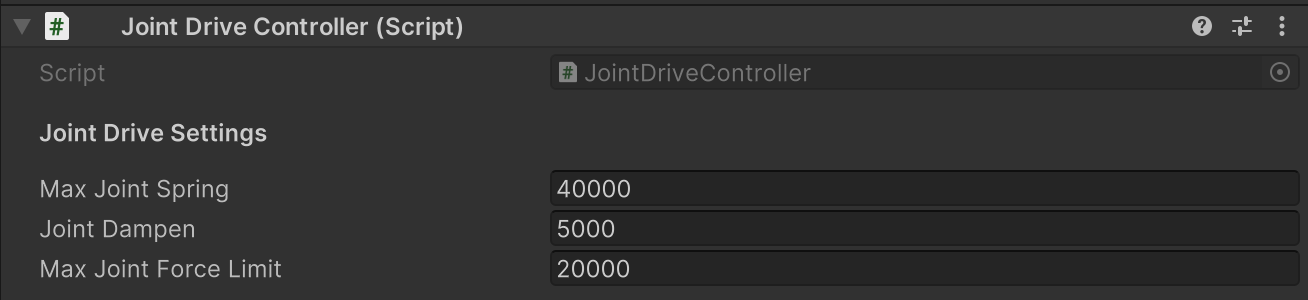
\includegraphics[scale=0.5]{img/gelenk_motor_steuerung.png}
  \caption{Gelenk Motor Steuerung}
  \label{fig:gelenk_motor_steuerung}
\end{figure}

\begin{itemize}
  \item Max Joint Spring: Bestimmt den Drehmoment mit welchem das Gelenk in die Zielposition rotiert wird.
  \item Joint Dampen: Verringert den Drehmoment proportional zur Differenz zwischen aktueller Geschwindigkeit und der Zielgeschwindigkeit. Verringert Schwingungen.
  \item Max Joint Force Limit: Gibt die maximale Kraft des Gelenks an (verhindert zu schnelle Bewegung bei großer Abweichung).
\end{itemize}


\section{Agent}
Das Walker Agent Skript, definiert den Läufer als Agent für das maschinelle Lernen. In Abbildung \ref{fig:agent_konfiguration} wird die Agentenkomponente im Inspektor gezeigt. Diese Komponente ist entscheidend für die Konfiguration der Lernumgebung des Läufers. Um die Komponente zu nutzen, müssen hier die Körperteile des Walkers referenziert werden. Diese Referenzierung ermöglicht es, spezifische Bewegungen und Interaktionen der einzelnen Körperteile zu steuern, was für das Training des Agenten entscheidend ist. Zusätzlich kann eine Zielgeschwindigkeit festgelegt werde und ob die Geschwindigkeit variieren soll während dem Training. Die Geschwindigkeit während dem Training zu variieren hilft dem Agent sein Verhalten besser an Umgebungsveränderungen anzupassen. Als letztes muss auch das Zielobjekt referenziert werden.

\begin{figure}[H]
  \centering  
  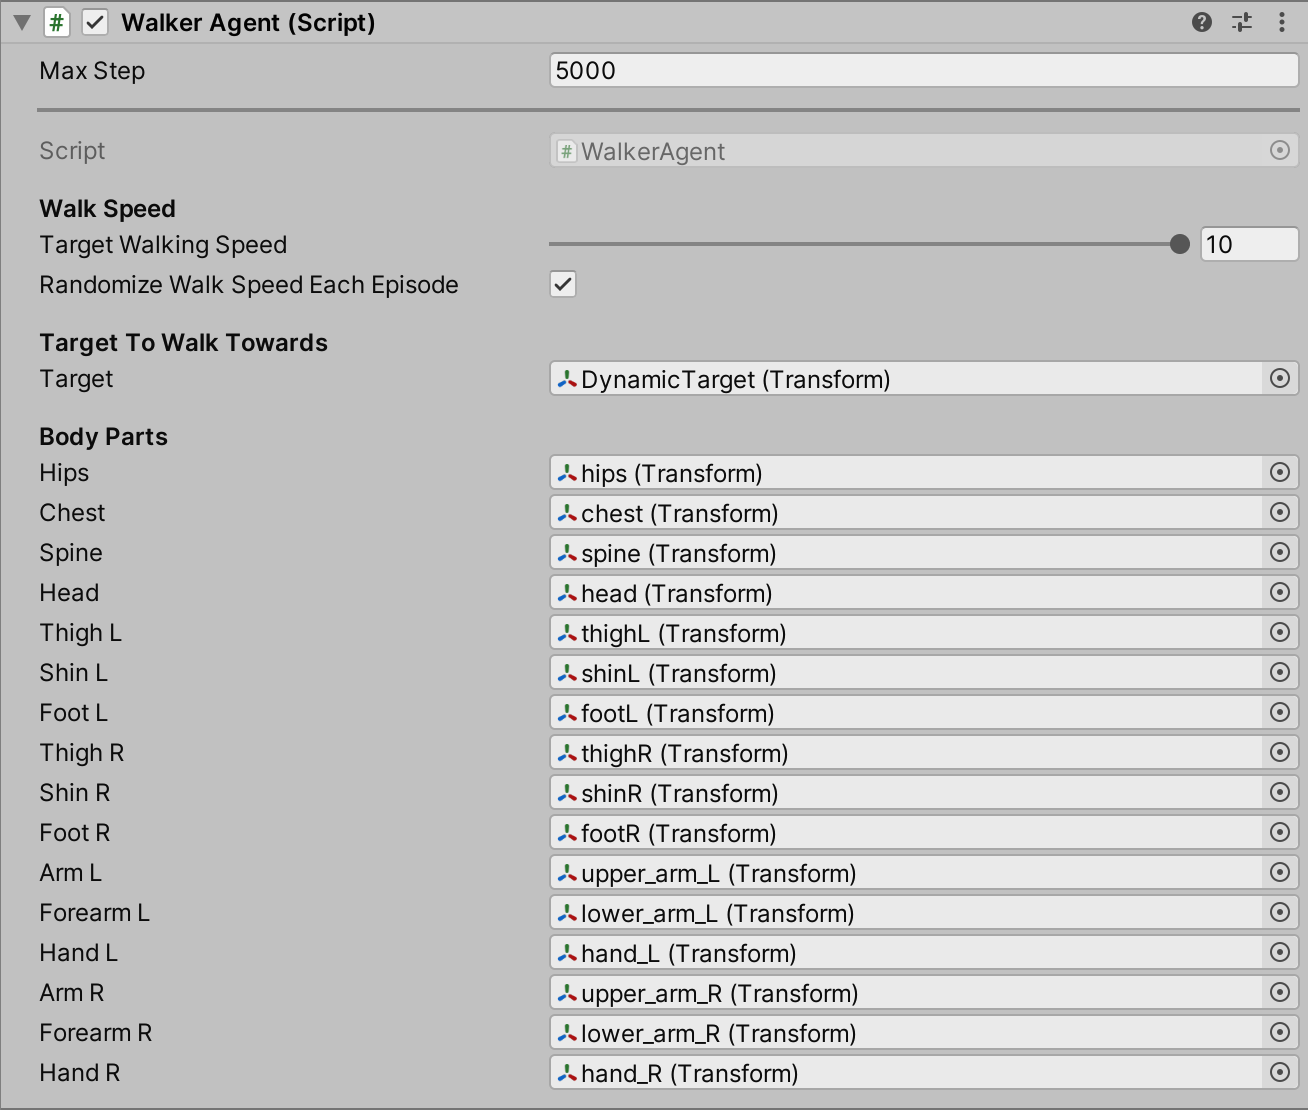
\includegraphics[scale=0.5]{img/agent_konfiguration.png}
  \caption{Agent Konfiguration}
  \label{fig:agent_konfiguration}
\end{figure}

Die Beobachtung des Agenten wird in Tabelle \ref{table:walker_beobachtung} dargestellt. Für jedes Körperteil wird die Beobachtung aus Tabelle \ref{table:walker_beobachtung_körperteil} dem Zustand angefügt. Die Beobachtungen müssen den Zustand des Läufers und der Umgebung im Bezug auf das Trainingsziel genau darstellen. Nur so kann der Agent die Situation verstehen und das Ziel erreichen.

\begin{table}[H]
  \centering
  {\rowcolors{1}{gray!10}{white}
  \begin{tabular}{ |p{1cm}|p{9cm}|p{5cm}|}
  \hline
  \textbf{ID} & \textbf{Beobachtung} & \textbf{Anmerkung}  \\
  \hline
  \rowids & Abweichung Durchschnittsgeschwindigkeit von Zielgeschwindigkeit &  \\
  \hline
  \rowids & Durchschnittsgeschwindigkeit &  \\
  \hline
  \rowids & Zielgeschwindigkeit & \\
  \hline
  \rowids & Abweichung Hüftrotation von Zielrotation & \\
  \hline
  \rowids & Abweichung Kopfrotation von Zielrotation & \\
  \hline
  \rowids & Zielposition & \\
  \hline
  \rowids & Körperteil Beobachtungen & Beobachtung aus Tabelle \ref{table:walker_beobachtung_körperteil} für jedes Körperteil \\
  \hline
  \end{tabular}}
  \caption{Walker Agent Beobachtung}
  \label{table:walker_beobachtung}
\end{table}
\rowidsclear

\begin{table}[H]
  \centering
  {\rowcolors{1}{gray!10}{white}
  \begin{tabular}{ |p{1cm}|p{9cm}|p{5cm}|}
  \hline
  \textbf{ID} & \textbf{Beobachtung} & \textbf{Anmerkung}  \\
  \hline
  \rowids & Bodenkontakt & \\
  \hline
  \rowids & Geschwindigkeit & \\
  \hline
  \rowids & Rotationsgeschwindigkeit & \\
  \hline
  \rowids & Position relativ zur Hüfte & \\
  \hline
  \rowids & LokaleRotation & Fehlt für Hüfte und Hände \\
  \hline
  \rowids & Gelenkstärke & Fehlt für Hüfte und Hände \\
  \hline
  \end{tabular}}
  \caption{Walker Agent Körperteil Beobachtung}
  \label{table:walker_beobachtung_körperteil}
\end{table}
\rowidsclear

Das Format einer Aktion besteht aus den in Tabelle \ref{table:walker_aktion} aufgeführten Feldern für jedes Körperteil des Läufers, ausgenommen der Hüfte und Hände. Jedes Körperteil wird somit separat bewegt, um die Bewegungen zu optimieren und schlussendlich das Gleichgewicht zu halten und das Fortbewegen zu erlernen.

Die Hüfte ist das zentrale Körperteil woran alle weiteren Körperteile mit Gelenken direkt oder indirekt anknüpfen. Aufgrund dieser zentralen Rolle wird die Hüftbeugung über das Gelenk des verbundenen Körpers gesteuert.

Da die Hände kaum Relevanz für das laufen haben, sind in der Demo fest mit dem Unterarm verbunden und brauchen daher nicht gesteuert werden.

\begin{table}[H]
  \centering
  {\rowcolors{1}{gray!10}{white}
  \begin{tabular}{ |p{1cm}|p{9cm}|p{5cm}|}
  \hline
  \textbf{ID} & \textbf{Beobachtung} & \textbf{Anmerkung}  \\
  \hline
  \rowids & Rotationswinkel X & Nur wenn Körperteil X Rotation beweglich ist\\
  \hline
  \rowids & Rotationswinkel Y & Nur wenn Körperteil Y Rotation beweglich ist\\
  \hline
  \rowids & Rotationswinkel Z & Nur wenn Körperteil Z Rotation beweglich ist\\
  \hline
  \rowids & Gelenkstärke & \\
  \hline
  \end{tabular}}
  \caption{Walker Agent Aktion}
  \label{table:walker_aktion}
\end{table}
\rowidsclear

Die Belohnungsfunktion enthält zwei Komponenten. Zum einen wird die Differenz der Bewegung in Zielrichtung zwischen momentaner Bewegung und Zielbewegung durch die Funktion $R_V$ bewertet. Somit wird der Läufer dazu motiviert effizient auf das Ziel zuzusteuern, indem Geschwindigkeit und Richtung optimiert werden. Zum Anderen wird die Abweichung zwischen momentaner Blickrichtung und der Zielrichtung in $R_L$ berechnet. Diese Komponente stellt sicher das der Läufer sich vorwärts geradeaus auf das Ziel bewegt. Die Belohnung ergibt sich am ende durch die Multiplikation beider Teilterme. Die Verwendung der Multiplikation hat zur Folge das die Belohnung gleichermaßen von beiden Teiltermen abhängig ist und es somit notwendig ist, beide Teile gleichzeitig zu optimieren. Als Ergebnis lernt der Läufer gleichermaßen die Ausrichtung als auch die Bewegung in Zielrichtung.

\begin{figure}[H]
  \centering  
  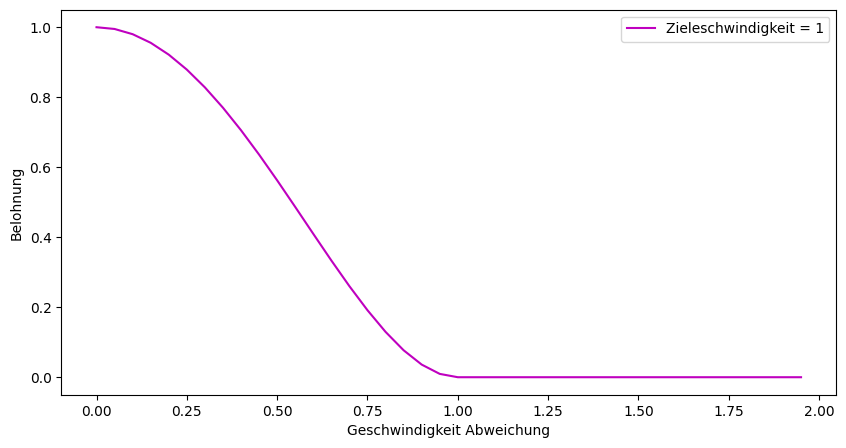
\includegraphics[scale=0.5]{img/match_velocity_demo_vel1.png}
  \caption{Walker Demo Match Velocity Belohnungsfunktion}
  \label{fig:match_velocity_demo_vel1}
\end{figure}

$V_\delta=Clip(|\vec{Geschwindigkeit} - \vec{Zielgeschwindigkeit}|, 0, |\vec{Zielgeschwindigkeit}|)$ \\
$R_V=(1 - (V_\delta / |\vec{Zielgeschwindigkeit}|)^2)^2$ \\

\begin{figure}[H]
  \centering  
  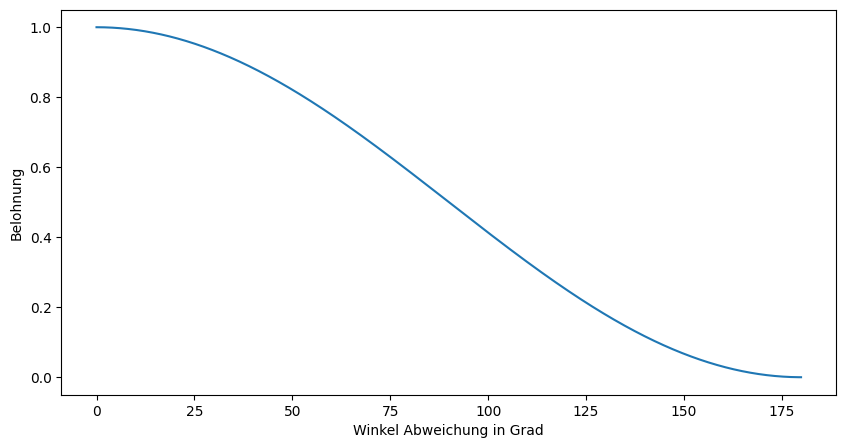
\includegraphics[scale=0.5]{img/look_at_target_demo.png}
  \caption{Walker Demo Look At Target Belohnungsfunktion}
  \label{fig:look_at_target_demo}
\end{figure}

$R_L=(\vec{Zielrichtung} \cdot \vec{Blickrichtung})+ 1) \cdot 0.5$ \\
$R=R_V \cdot R_L$

Initialisierung bzw Episodereset erklären
Orientation Object erklären
Zielsetzung erklären
Rewardfrequenz erwähnen